\documentclass{cheatsheet}
\usepackage{bm}
\usepackage{textcomp, mathcomp}
\usepackage{empheq}
\usepackage{pbox}
\usepackage{booktabs}
\usepackage{verbatim}

\doctitle{... Cheatsheet}
\author{AUTHOR \\ \vspace*{-0.2em}}

\begin{document}
\section{1. Terminology}
	\subsection{1.1 Input, Output, State}
    %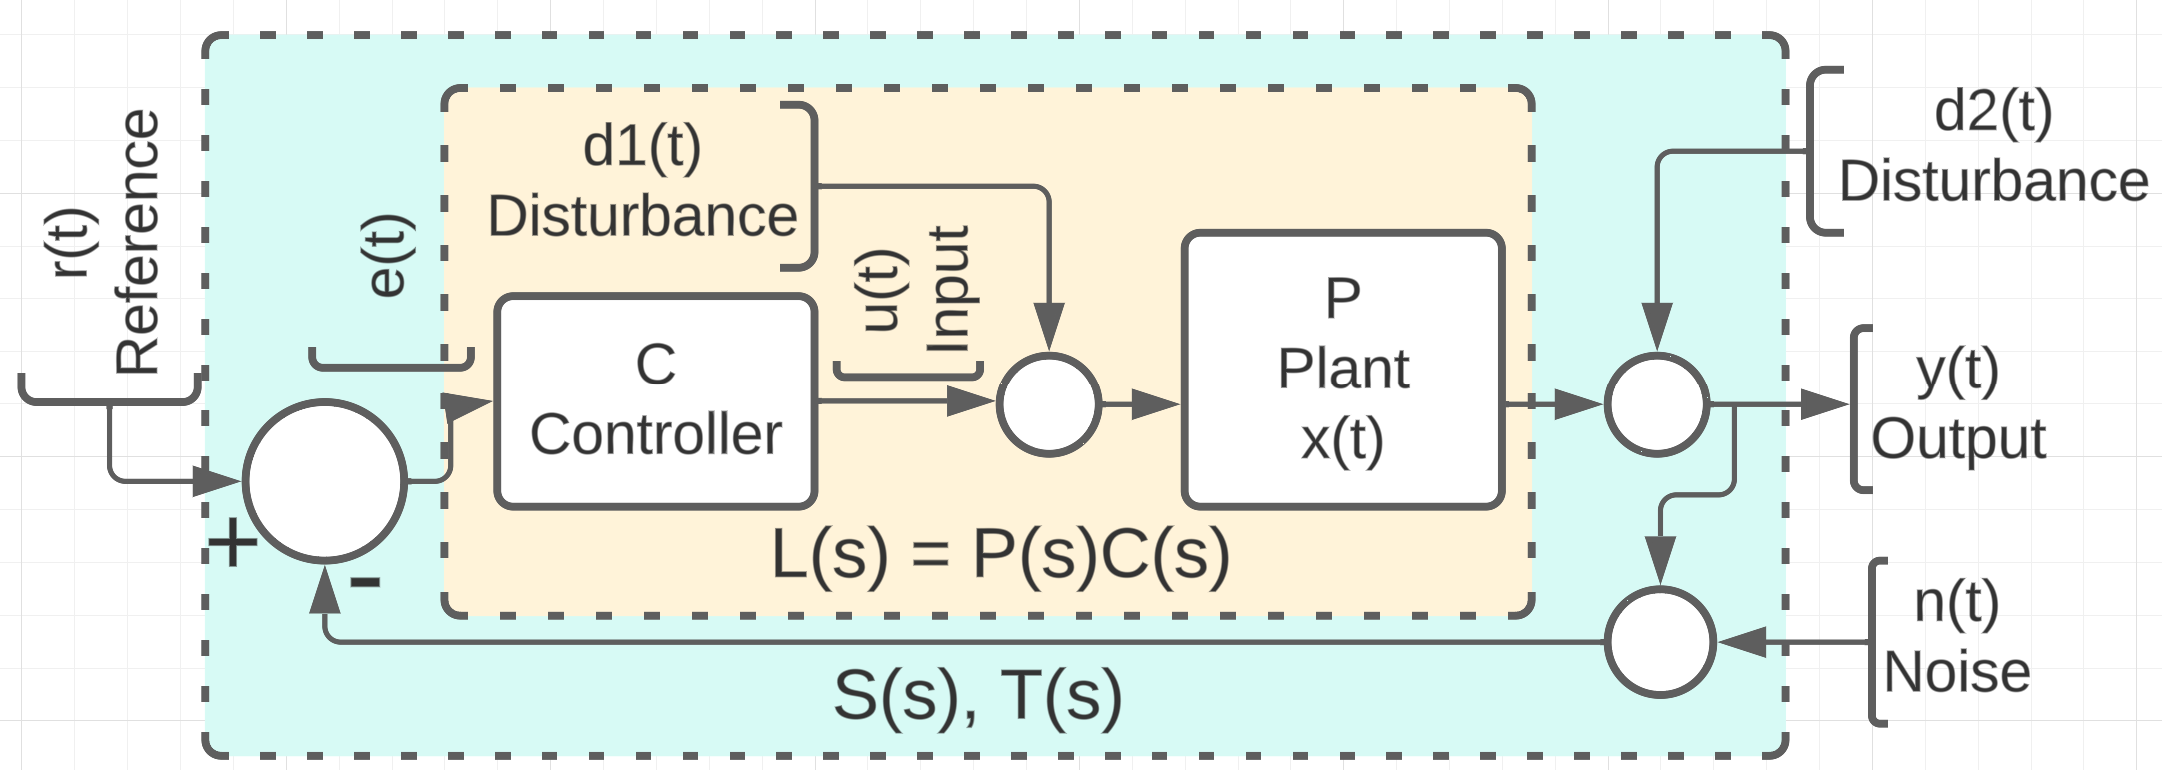
\includegraphics[width = \linewidth]{src/images/basic_block_chart.png}
    \begin{itemize}
        \item \textbf{(Control) Input u(t)} (gas pedal)
        \begin{itemize}
            \item endogenous: manipulation by designer
            \item exogenous: generated by environment (e.g. Weather)
        \end{itemize}
        \item \textbf{Output / Measurement y(t)} (speed)
        \begin{itemize}
            \item measured outputs: Quantities that we can measure
            \item performance outputs: unmeasurable but controllable (e.g. average fuel consumption)
        \end{itemize}
        \item \textbf{state x(t)}: "memory", summary of all past inputs (fuel)
        \item parameter: quantities that do not change over time (colour)
\end{itemize}
	\subsection{State Space Form}
    \begin{minipage}{0.49 \linewidth}
        \begin{center}
            \textbf{\underline{General form}}
        \end{center}
        \begin{align*}
            \begin{cases}
                \dot{x}(t) = f(x(t), u(t), d(t))\\
                y(t) = f(x(t), u(t), d(t))
            \end{cases}
        \end{align*}
    \end{minipage}
    \begin{minipage}{0.49 \linewidth}
        \begin{center}
            \textbf{\underline{Linear System}}
        \end{center}
        \begin{align*}
            \begin{cases}
                \dot{x}(t) = Ax(t) + Bu(t)\\
                y(t) = Cx(t) + Du(t)
            \end{cases}\\
        \end{align*}
    \end{minipage}
    dim$(x) = $ Order/Dimension (min. $\#$ of variables to describe state)
    
	\subsection{Systems}
    LTI: Linear time-invariant system (y(t) ~ u(t))\\
    SISO: Single input single output system
	\subsection*{Classification}
    \subsubsection*{LTI-Systems}
        Linear vs Nonlinear:
        System can be represented in state-space-form:
        \begin{equation}\label{eqn:LTI}
            \begin{cases}
                \dot{x}(t) = Ax(t) + Bu(t)\\
                y(t) = Cx(t) + Du(t)
            \end{cases}
        \end{equation}
        -> linear system -> superposition can be used\\
        $y(t) = f(au_1(t)+bu_2(t)) = af(u_1(t)) + bf(u_2(t))$
    
    \subsubsection*{Causal systems}
        Causal vs Non-Causal:
        Output at time $t$ depends only on inputs that happened before and not after $t$ (future inputs do not affect current output)\\
        $y(t) = f(u(\tau)), \tau < t$
    
    \subsubsection*{Static systems}
        Static (memoryless) vs Dynamic
        y(t) only depends on u(t), output does not depend on past or future\\
        $dim(x) = 0$ : dimension of system equals 0

    \subsubsection*{Time invariant vs Time-varying}
        output does not depend on time, only on $\Delta t$ (counter example sun clock)\\
        {\centering\textbf{\underline{Time-varying}}}
        \begin{equation}
            t_0 = t_0
            \begin{cases}
                \dot{x}(t) = f(t, x(t), u(t))\\
                y(t) = g(t, x(t), u(t))
            \end{cases}
            \rightarrow
            \begin{cases}
                \dot{x}(t) = A(t)x(t) + B(t)u(t)\\
                y(t) = C(t)x(t) + D(t)u(t)
            \end{cases}
        \end{equation}

        {\centering\textbf{\underline{Time Invariant}}}
        \begin{align*}
            \sigma_{\tau} y(t) = \sum \sigma_{\tau} u(t)\\
            y(t - \tau) = \sum(u(t - \tau))\\
            t_0 = 0
            \begin{cases}
                \dot{x}(t) = f(x(t), u(t))\\
                y(t) = g(x(t), u(t))
            \end{cases}
            \rightarrow
            \begin{cases}
                \dot{x}(t) = Ax(t) + Bu(t)\\
                y(t) = Cx(t) + Du(t)
            \end{cases}
        \end{align*}
	\subsection{Interconnections}
    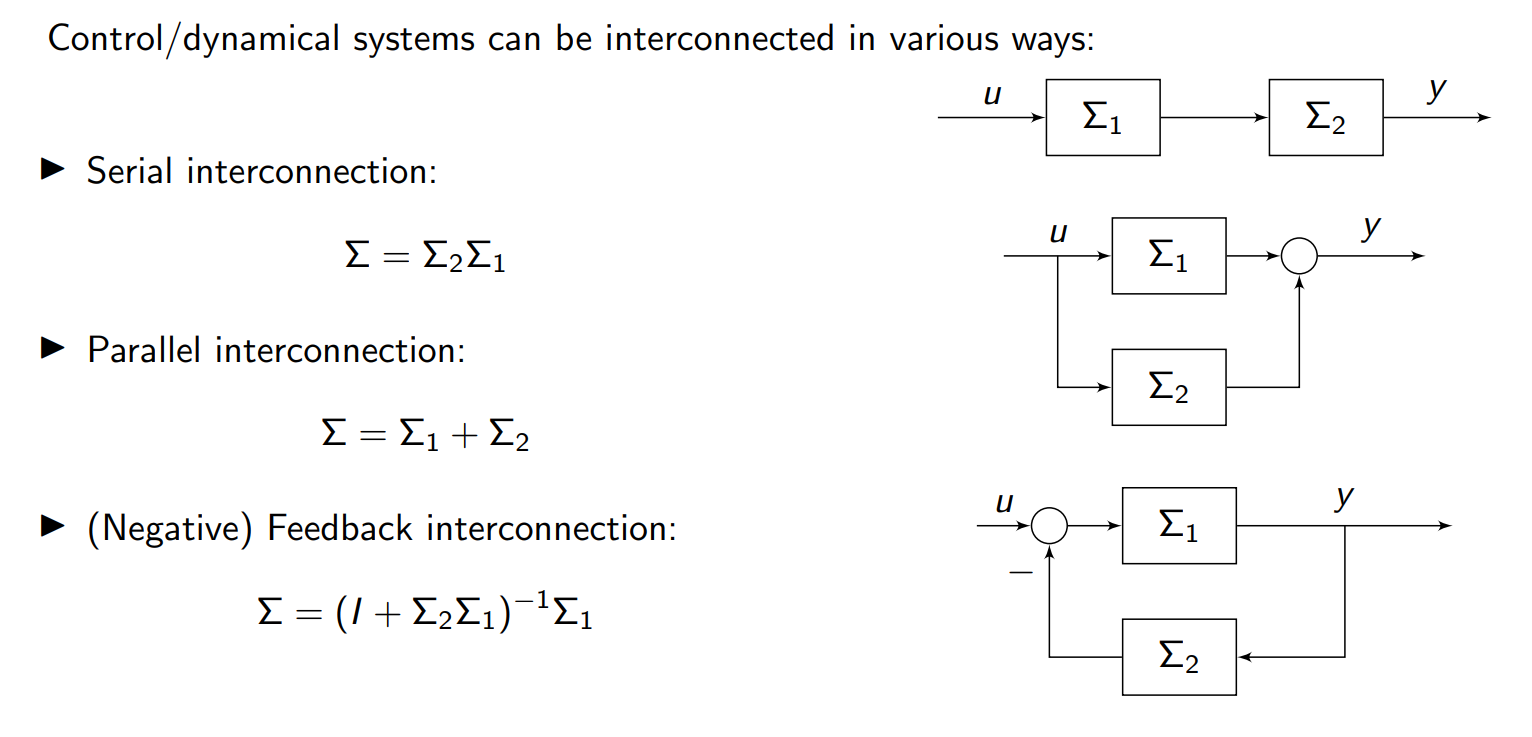
\includegraphics[width = \linewidth]{src/images/interconnection.png}
	\subsection{Basic Control Architectures}
    \begin{tabu}{X[m] X[2, c, m]}
        \textbf{Name}               & \textbf{Block chart}\\
        \hline \hline
        Feed-forward      & 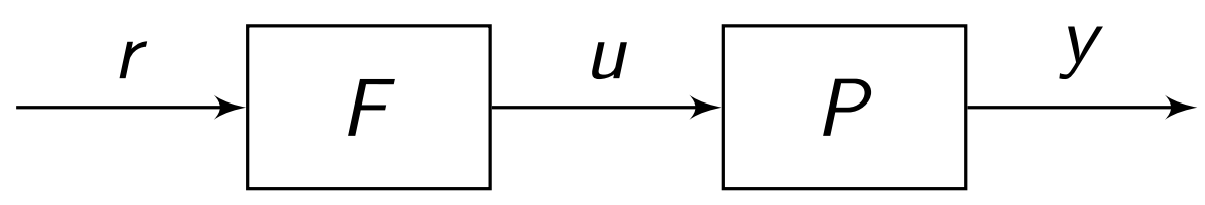
\includegraphics[width = \linewidth]{src/images/architecture_feed_forward.png}\\
        \hline
        Feedback    & 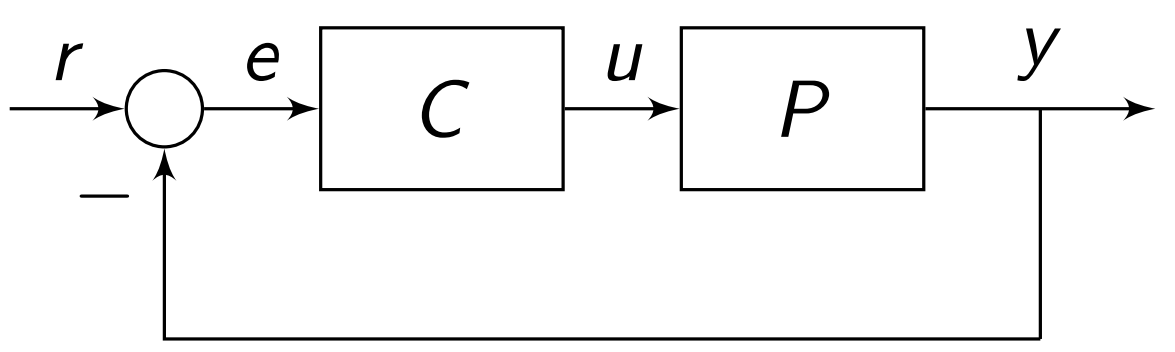
\includegraphics[width = \linewidth]{src/images/architecture_feedback.png}\\
        \hline
        Two degrees of freedom    & 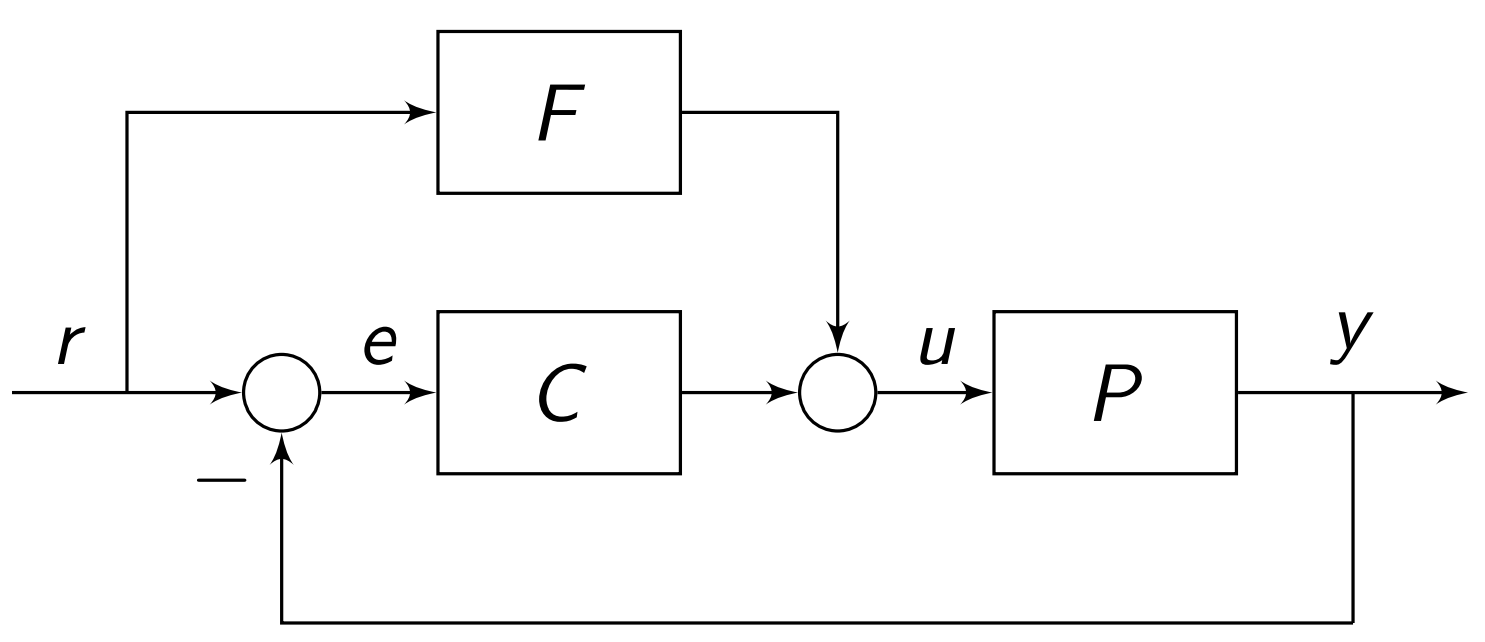
\includegraphics[width = \linewidth]{src/images/architecture_two_freedom.png}
    \end{tabu}
	\subsection*{Mechanical Systems}
    
	\subsection*{Thermodynamic Systems}
    $C_i \cdot T_i = (Q_j - Q_k)$
    $\dot{Q}_a = c_a(T_i - T_j)$

\section{2. System Modeling}
	for LTI SISO systems: $\frac{d}{dt} \text{storage} = \sum \text{inflows} - \sum \text{outflows}$

    \begin{center}
        \textbf{\underline{Mass conservation}}    
    \end{center}
    \begin{align*}
        \frac{d}{dt} m = \sum m_{in}(t) - \sum m_{out}(t)
    \end{align*}

    \begin{center}
        \textbf{\underline{Mechanical systems}}    
    \end{center}
    \begin{align*}
        M(t) = J \cdot \ddot{\phi}(t)
    \end{align*}

    \begin{center}
        \textbf{\underline{Thermodynamic systems}}    
    \end{center}
    \begin{align*}
        m \frac{d}{dt} T(t) = c(T_{ext}(t) -T(t)) + u(t)
    \end{align*}
	

\section{2. linearization process}
	\subsection*{Jacobian Linearization Process}
    Use in LTI-Systems, see equation \ref*{eqn:LTI}
    \begin{align*}
        \left(
            \begin{array}{c}
                x\\
                u
            \end{array}
        \right)
        =
        \left(
            \begin{array}{c}
                x_e\\
                u_e
            \end{array}
        \right)
    \end{align*}
    \begin{align*} % \Big\rvert_{x = x_e, u = u_e} Auswertung der Differentiale
        A &= 
        \left[\begin{array}{c c c}
            \frac{\partial f_1}{\partial x_1} & \cdots & \frac{\partial f_1}{\partial x_n}\\
            \vdots & \ddots & \vdots\\
            \frac{\partial f_n}{\partial x_1} & \cdots & \frac{\partial f_n}{\partial x_n}
        \end{array}\right]
        &B &= 
        \left[\begin{array}{c}
            \frac{\partial f_1}{\partial u}\\
            \vdots\\
            \frac{\partial f_n}{\partial u}
        \end{array}\right]
        \\
        C &= 
        \left[\begin{array}{c c c}
            \frac{\partial g}{\partial x_1} & \cdots & \frac{\partial g}{\partial x_n}
        \end{array}\right]
        &D &= 
        \left[\begin{array}{c}
            \frac{\partial g}{\partial u}
        \end{array}\right]
    \end{align*}
\end{document}

\begin{comment}
	TERMINOLOGY
	Definitions from ZF
Input, output, state…
	Classification of Systems (Also see ZF)
SYSTEM MODELING / transfer real world problems to input output system
	Thermodynamics
	Conservation of mass: for LTI SISO systems: $\frac{d}{dt} \text{storage} = \sum \text{inflows} - \sum \text{outflows}$

	Mechanics
NETWORK ANALYSIS
	(Interconnections & Basic Control Architectures) (Block Diagrams on ZF)
LINEARIZATION
	Jacobian Linearization process
LINEAR SYSTEM ANALYSIS
TIME RESPONSE
STABILITY
	Equilibrium point: $\dot{x}(t) = 0
FREQUENCY DOMAIN
	y(t) = G(s) * u(t) for u(t) = e^(st)
	Therefore, for sinusoidal inputs: u(t) = cos(omega * t) -> y = M cos(omega * t + phi), M = |G(j * omega)|, phi = \angle G(j * omega
	e^(i*s*t) = cos(s*t) + i*sin(s*t), cos(s*t) = 
	STATE SPACE -> TRANSFER FUNCTION
	TRANSFER FUNCTION -> CONTROLLABLE CANONICAL FORM
	POLES/ZEROS
SIMPLE LAPLACE
	derivative of a laplace function
	laplace of step function
	laplace of x^n
\end{comment}